\chapter{Map-Based Comparison Using HEALPix}

The objective of this chapter is to project the instrumental noise onto the sky by generating noise maps that highlight the spatial manifestation of temporal noise correlations. By implementing a longer simulation, we can examine how $1/f$ drifts translate into systematic patterns on the celestial sphere. Furthermore, this approach allows us to perform an angular power spectrum analysis by decomposing the resulting maps into spherical harmonics.

\section{Long-Term Simulations}

The analysis conducted in Chapter 5 validated the noise models on short timescales ($10^3$~s). However, to evaluate the scientific impact of instrumental noise on cosmological observations, it is necessary to extend the simulation to timescales comparable to the actual mission duration.

$1/f$ noise is intrinsically correlated in time. During scanning operations, the telescope's scanning strategy projects these temporal correlations onto the celestial sphere. While white noise distributes itself uniformly and independently across pixels, the low-frequency fluctuations of correlated noise (drifts) act over long periods, affecting sequences of pixels observed consecutively along the scanning path. This effect typically results in stripes on the final maps.

Only through long-duration simulations can we ensure that the same region of the sky is scanned multiple times with different crossing angles and at different epochs. This process is fundamental for averaging down temporal drifts and ensuring full sky coverage; specifically, a one-year simulation ensures that the scanning strategy covers the entire area of interest with a statistically significant number of hits per pixel.

For this analysis, the setup for the custom detector (summarized in Table 5.1) was maintained. The decision to not use the IMo detector at this stage was driven by the need to emphasize the $1/f$ components. The higher $f_{\text{knee}}$ of the custom model makes the resulting noise patterns more visually and statistically evident in the maps, providing a robust test for the map-making pipeline.

The key parameters for the long-term simulation are:
\begin{itemize}
    \item Total duration: $T_{\text{obs}} = 365$ days ($\approx 3.15 \times 10^7$~s).
    \item Sampling frequency: $f_{\text{samp}} = 20$~Hz.
    \item Total samples: $N_{\text{tot}} = T_{\text{obs}} \cdot f_{\text{samp}} = 630,720,000$.
    \item Noise segmentation: noise generation is divided into 12-hour blocks ($43,200$~s). This scale is sufficiently long to capture all relevant frequencies above $f_{\text{min}}$, while remaining computationally manageable for the generation algorithms.
\end{itemize}

Managing over 600 million samples presents significant computational challenges. Allocating a NumPy array of this size would require approximately 5~GB of RAM for a single detector. Considering that a real mission involves thousands of detectors, the standard approach---loading the entire Time-Ordered Data (TOD), processing it, and then projecting it---becomes impractical. Furthermore, performing a Fast Fourier Transform (FFT) on an entire year of data would impose prohibitive memory requirements and execution times.

To overcome these limitations, an incremental map-making pipeline was implemented:
\begin{enumerate}
    \item The total observation time is partitioned into 12-hour chunks.
    \item For each chunk, the pointing sequences and the corresponding noise TOD are generated on-the-fly.
    \item The data are immediately projected onto the HEALPix map, and the TOD samples are subsequently cleared from memory to free up resources.
    \item The final map is obtained at the end of the cycle by normalizing the accumulated signal by the hit count per pixel.
\end{enumerate}




\section{Map-Making Procedure}

The process of projecting data from the time domain to the spatial domain (maps) represents a fundamental stage of the analysis pipeline. In this work, two types of HEALPix maps were produced for each simulation: a hit-map and a noise-only map.

The hit-map is a map of integers where each pixel contains the total number of samples ($N_p$) that fell within its boundaries during the full year of scanning. This map serves as the metric of the observation: it measures sky coverage, identifies frequently observed regions versus those with lower exposure, and is essential for properly normalizing and averaging the time-domain signal. It is important to note that the hit-map is independent of the presence of noise; it depends exclusively on the scanning strategy and the telescope's pointing geometry.

The noise-only maps contain the generated noise signal. No astronomical signals (CMB or foregrounds) were included in these simulations. This choice aims to isolate the instrumental noise contribution exclusively. In a real-world map, $1/f$ noise is blended with CMB anisotropies; by producing noise-only maps, we can directly visualize the texture produced by temporal correlations and quantify the residual uncertainty that would affect scientific data.

For map production, a binned map-making algorithm was employed. In this configuration, the value of a pixel $m(p)$ is calculated as the simple average of all TOD samples falling into that specific pixel:

\begin{equation}
m(p) = \frac{1}{N_p} \sum_{i \in \text{pixel } p} d_i
\end{equation}

where $d_i$ represents a single TOD sample and $N_p$ is the corresponding value in the hit-map for pixel $p$.

The absence of filtering or pre-processing allows the large-scale structures produced by $1/f$ noise to be fully exposed. This is essential for comparing the \texttt{add\_lbsNoise} and \texttt{add\_OofaNoise} models, as a destriping algorithm would likely mask the very differences we aim to analyze.

In a standard cosmological analysis, this procedure would typically be followed by a destriping phase. Destripers are algorithms designed to suppress the stripes caused by $1/f$ drifts. Although the LBS framework includes an implemented destriping module, it was not utilized in this work. The algorithm is extremely demanding in terms of memory and processing power, as it requires solving large linear systems (one equation per pixel or scanning basket), which exceeded the computational resources available for this study.

In the end, the map resolution is determined by the \texttt{nside} parameter. For this work, $N_{\text{side}} = 2^7 = 128$ was chosen, resulting in a total of $196,608$ pixels on the sphere ($N_{\text{pixel}} = 12N_{\text{side}}^2$). While high-resolution studies typically use $N_{\text{side}} = 512$, the choice of a lower value is justified by the fact that at high resolutions, white noise would visually dominate individual pixels, obscuring large-scale correlations. At $N_{\text{side}} = 128$, the characteristic stripes induced by the temporal correlations of $1/f$ noise become clearly distinguishable, facilitating a qualitative and quantitative comparison between the models.




\section{Memory Optimization and Performance}

Projecting a full year of data onto a HEALPix map presents significant computational challenges for standard Python environments. With over 600 million samples to process, the analysis would be restricted to timescales too short to be scientifically meaningful without dedicated optimization.

In Python, iterating through large-scale arrays using standard \texttt{for} loops is notoriously slow. During initial testing without optimization, simulations were limited to a maximum of 60 days of observation. However, 60 days is insufficient to guarantee the complete and uniform sky coverage required by the LiteBIRD scanning strategy.

So the Numba\footnote{\url{https://numba.pydata.org/}} library was employed. By utilizing the \texttt{@njit} (No-Python Just-In-Time) decorator, critical functions are compiled into highly optimized machine code at runtime.

Specifically, two optimized procedures were implemented to operate directly on memory buffers:
\begin{itemize}
    \item Sample Accumulation: this function performs a loop over detectors and time samples. For each time step, it retrieves the corresponding pixel index from the pointing vector and simultaneously updates two maps: it adds the signal value to the accumulation map and increments the counter in the hit-map by one.
    \item Final Normalization: once the processing of all temporal blocks is complete, this procedure iterates through the entire HEALPix map. For every pixel visited at least once (i.e., where the hit-map value is greater than zero), it calculates the average noise value by dividing the accumulated signal by the number of observations ($N_p$).
\end{itemize}

The implementation of these optimized functions enabled the processing of a full year of simulation data. This, in turn, allowed for complete sky coverage, which is essential for investigating the spatial stripping patterns induced by $1/f$ noise.




\section{Analysis of Noise Maps}

This section presents a qualitative analysis of the HEALPix maps generated by the two noise models: \texttt{add\_lbsNoise} (Figure 6.1) and \texttt{add\_OofaNoise} (Figure 6.2). 

The resulting maps reveal an overlap of two distinct morphological patterns:
\begin{itemize}
    \item Fine-grained fluctuations (White Noise): an isotropic, small-scale random fluctuation is visible in the background. This represents the white noise contribution, which lacks spatial correlations and is distributed independently across pixels.
    \item Striations ($1/f$ Noise): superimposed on the fine-grained background, clear stripes emerge. These striations are the characteristic signature of $1/f$ noise; since the noise is temporally correlated, pixels observed consecutively along the telescope's line of sight tend to share similar values (consistently higher or lower than the mean), creating coherent large-scale structures.
\end{itemize}

The color scales of the maps provide essential quantitative insights. The hit-map shows a non-uniform coverage, with two high-density horizontal bands (peaking at approximately $8,894$ hits per pixel) where the scanning strategy focuses most frequently. In the noise maps, the values are on the order of $10^{-5}$~K (tens of $\mu\text{K}_{\text{CMB}}$), confirming that the noise amplitude is consistent with the detector's NET. The distribution is nearly symmetric around zero, indicating that the generated noise correctly fluctuates without a systematic bias.

A comparison between the \texttt{add\_lbsNoise} and \texttt{add\_OofaNoise} maps reveals strong statistical consistency. Both models faithfully reproduce the same striation texture, and the ranges of minimum and maximum values are remarkably similar. This demonstrates that despite different internal implementations, the total noise power and its projection onto the sphere are correctly preserved by both methods. 

\begin{figure}[h!]
    \centering
    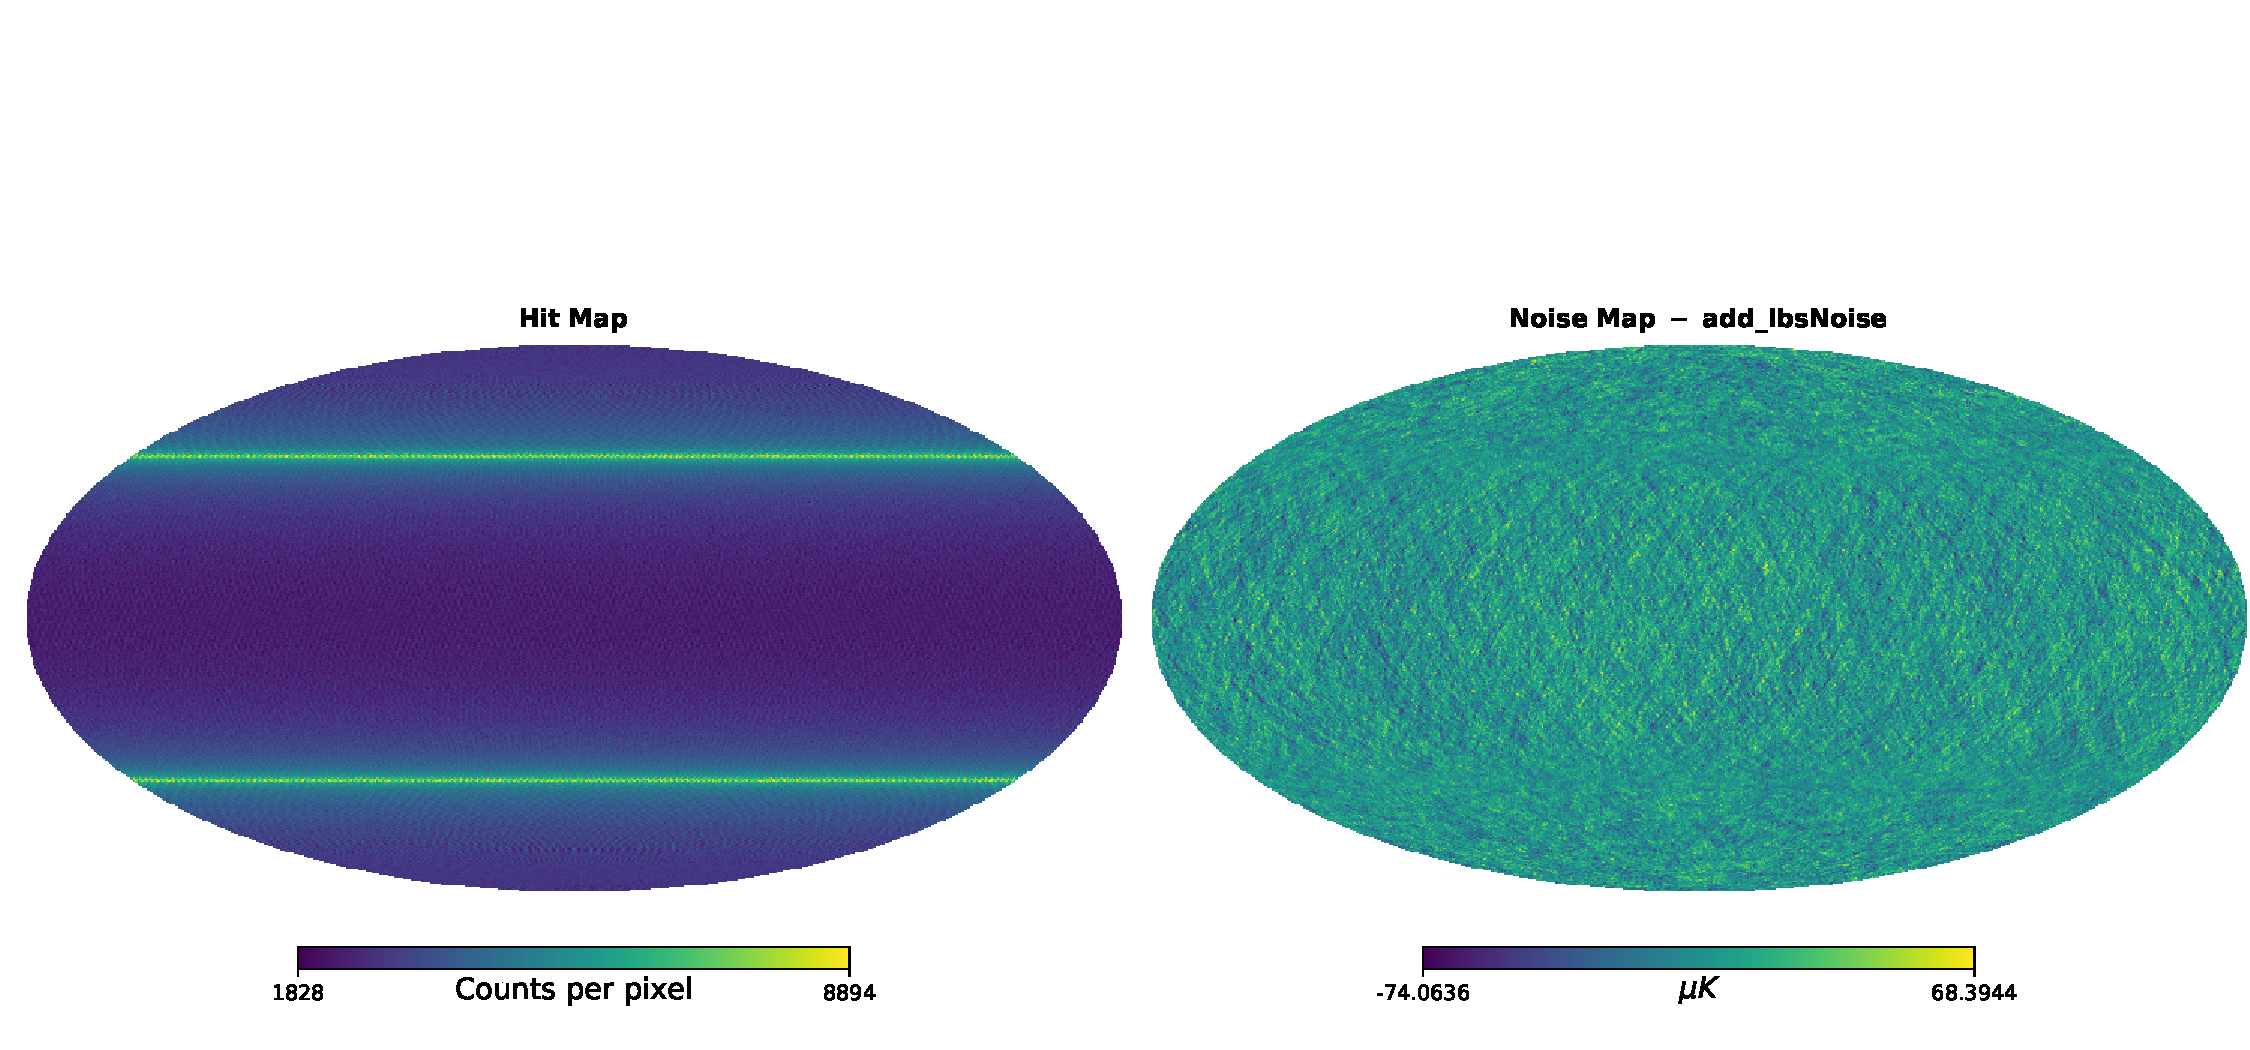
\includegraphics[width=0.8\textwidth]{map_lbs.pdf}
    \caption{HEALPix map using \texttt{add\_lbsNoise}.}
    \label{fig:map_lbs}
\end{figure}

\begin{figure}[h!]
    \centering
    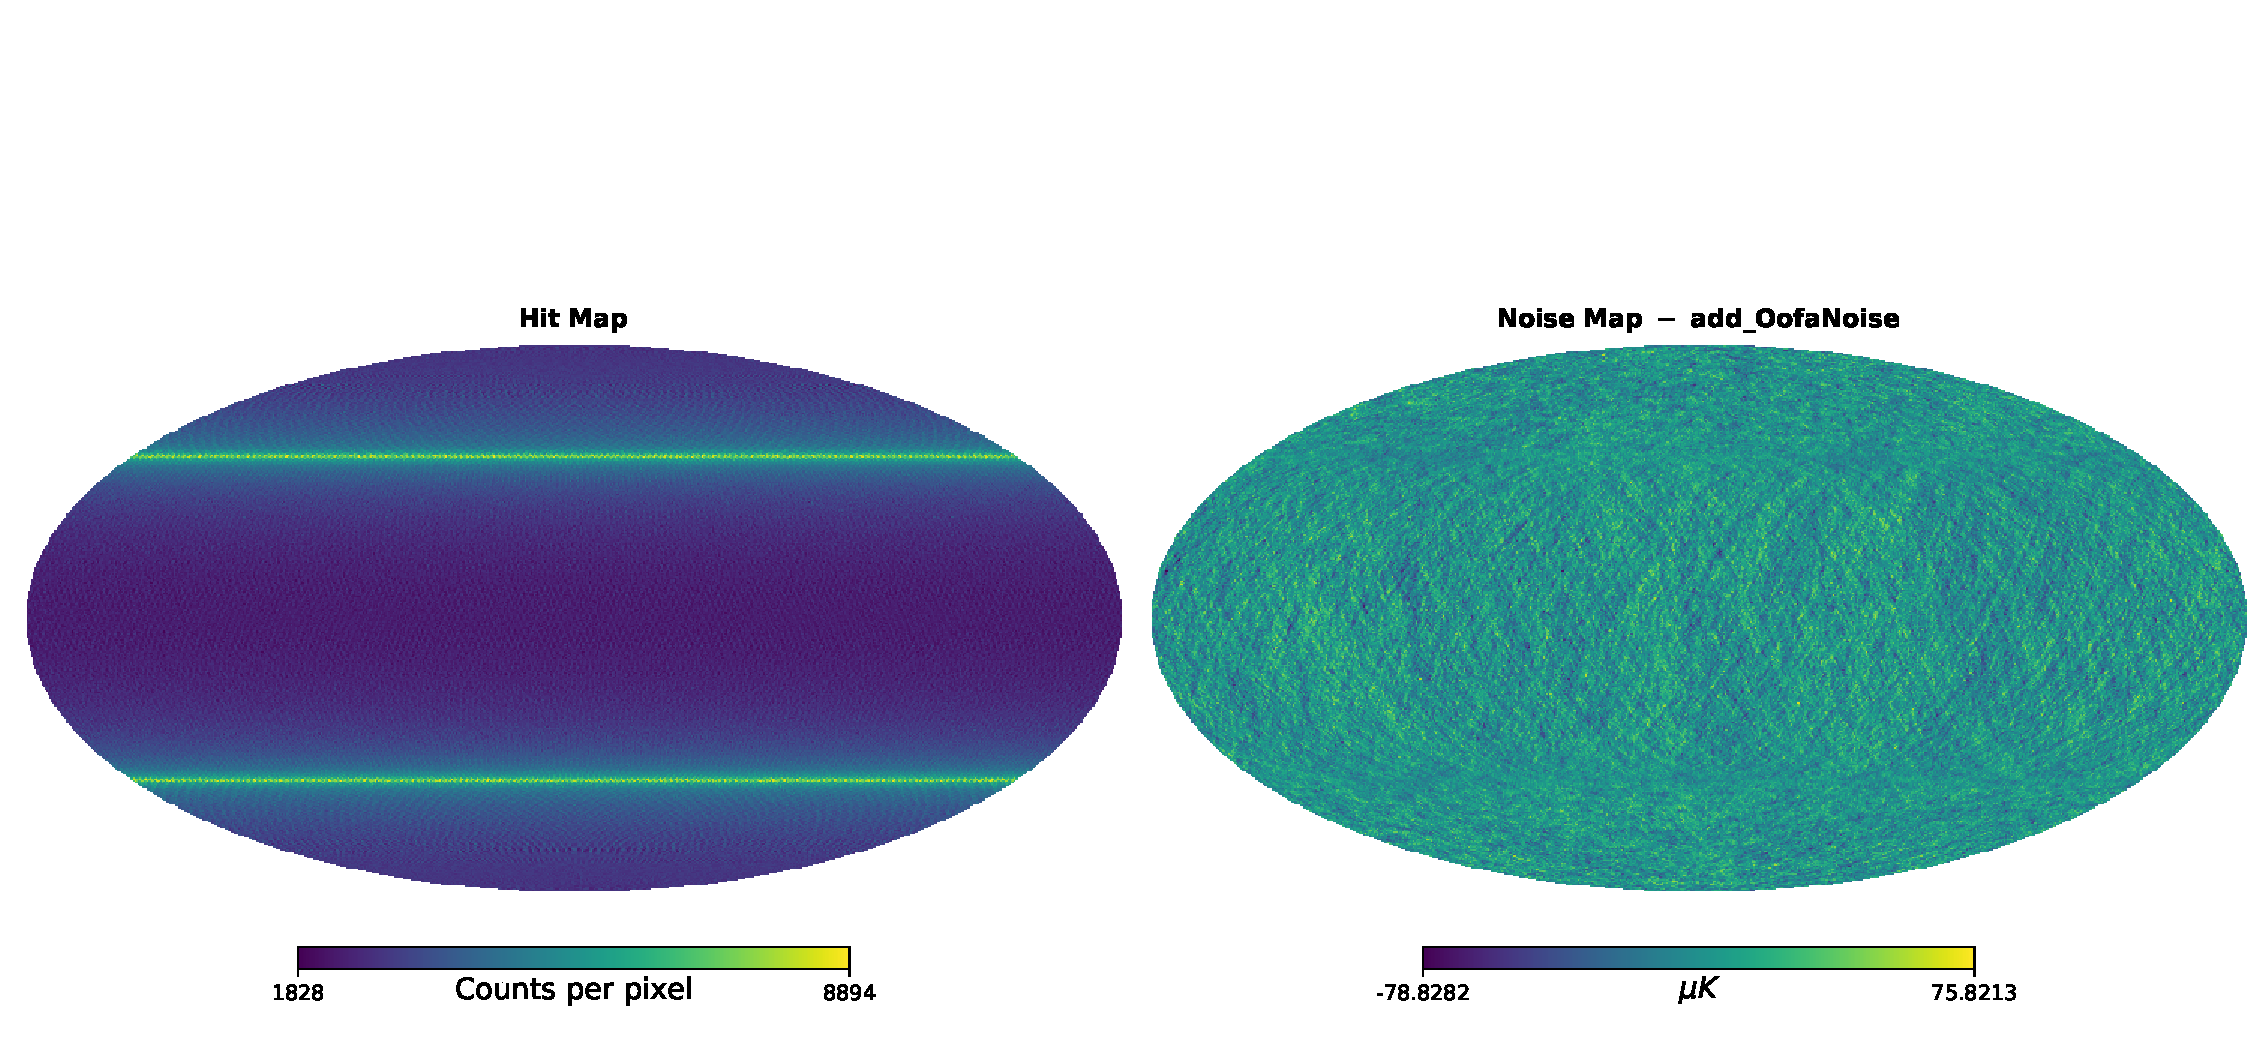
\includegraphics[width=0.8\textwidth]{map_oofa.pdf}
    \caption{HEALPix using \texttt{add\_OofaNoise}.}
    \label{fig:map_oofa}
\end{figure}

An interesting observation concerns the noise uniformity across the celestial sphere. While striations are visible globally, the noise pattern appears more blurred or attenuated in regions frequently visited by the satellite (the brighter bands in the hit-map). This phenomenon is a direct consequence of LiteBIRD's scanning redundancy. When a pixel is observed a high number of times, there is a statistical cancellation of drifts. Different scanning segments crossing the same pixel at distant intervals carry independent noise drifts. 

However, it is important to distinguish the behavior of correlated noise from that of white noise. For a pure white noise signal with a standard deviation in the TOD of $\sigma \approx 220~\mu\text{K}$, a one-year integration (corresponding to approximately $3200$ hits per pixel at $N_{\text{side}}=128$) would reduce the residual noise to $\sigma/\sqrt{N_p} \approx 4~\mu\text{K}$. In contrast, the noise maps generated in this work exhibit fluctuations on the order of tens of $\mu\text{K}$.

This demonstrates that $1/f$ noise does not average down as efficiently as white noise. Because $1/f$ fluctuations possess long-term correlations, the drifts do not cancel out completely even with high redundancy; instead, they leave a residual systematic signal that remains significantly higher than the theoretical white noise limit. This confirms that, while the geometric structure of the scanning strategy acts as a primary natural filter for correlated noise, it cannot fully substitute for dedicated numerical destriping algorithms in preserving the scientific integrity of the maps.

Conversely, in low-density regions where the satellite makes fewer passes, the contrast of individual stripes remains sharp, making the $1/f$ noise much more prominent. This confirms that, even in the absence of numerical destriping algorithms, the geometric structure of the scanning strategy itself acts as a primary, natural filter for correlated noise.




\section{Harmonic-Domain Analysis of Noise Maps}

The final characterization of the noise is conducted in the harmonic domain. This step is essential to quantify the impact of temporal correlations across different angular scales and to statistically validate the consistency between the implemented noise models.

Since the detectors simulated in this work are configured to measure total intensity only, the analysis is restricted to temperature maps ($T$). The spatial domain signal $m(\hat{n})$ is decomposed into the spherical harmonics basis $Y_{\ell m}(\hat{n})$:

\begin{equation}
m(\hat{n}) = \sum_{\ell=0}^{\ell_{\text{max}}} \sum_{m=-\ell}^{\ell} a_{\ell m} Y_{\ell m}(\hat{n})
\end{equation}

From the resulting amplitudes $a_{\ell m}$, the auto-correlated angular power spectrum ($TT$) is calculated:

\begin{equation}
C_\ell^{TT} = \frac{1}{2\ell+1} \sum_{m=-\ell}^{\ell} |a_{\ell m}|^2
\end{equation}

This quantity represents the noise power as a function of the multipole $\ell$, where low $\ell$ values correspond to large angular scales and high $\ell$ values to small angular scales. It should be noted that computing cross-polarized spectra ($EE, BB$) or cross-correlations ($TE$) would require defining the polarization angle for each detector.

A crucial aspect for the validation of this work is the correspondence between the Power Spectral Density in the time domain and the angular power spectrum ($C_\ell$) on the sphere. When generating a map containing only white and $1/f$ noise, the $C_\ell$ trend mirrors the Time-Ordered Data (TOD) properties according to the relation:

\begin{equation}
C_\ell \propto \sigma^2 \left[ 1 + \left( \frac{\ell_{\text{knee}}}{\ell} \right)^\alpha \right]
\end{equation}

In this expression, $\ell_{\text{knee}}$ represents the knee multipole, the spatial equivalent of the temporal knee frequency ($f_{\text{knee}}$). This similarity is not accidental; it reflects how the scanning strategy projects the detector's temporal fluctuations onto the angular scales of the sky. 

For this analysis, we set $\ell_{\text{max}} = 3N_{\text{side}} - 1 = 383$. The choice of $N_{\text{side}}=128$ determines the angular resolution of the map, resulting in a pixel size of approximately $27.5'$, or just under half a degree. Given that the angular scale $\theta$ is approximately related to the multipole by $\ell \approx 180^\circ / \theta$, $\ell \approx 180$ corresponds to degree scales. With the current resolution, the spectrum is reliable up to $\ell \approx 350$.

\begin{figure}[h!]
    \centering
    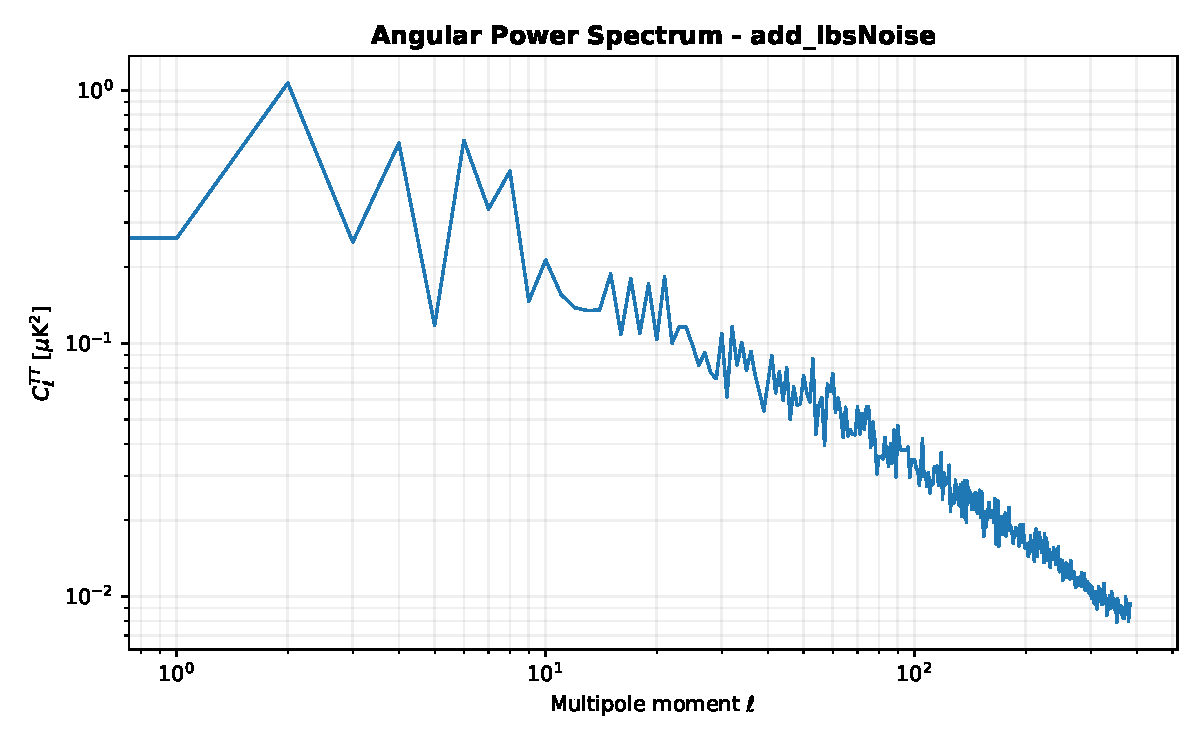
\includegraphics[width=0.65\textwidth]{psd_sh_lbs.pdf}
    \caption{Angular power spectrum using \texttt{add\_lbsNoise}.}
    \label{fig:psd_sh_lbs}
\end{figure}

\begin{figure}[h!]
    \centering
    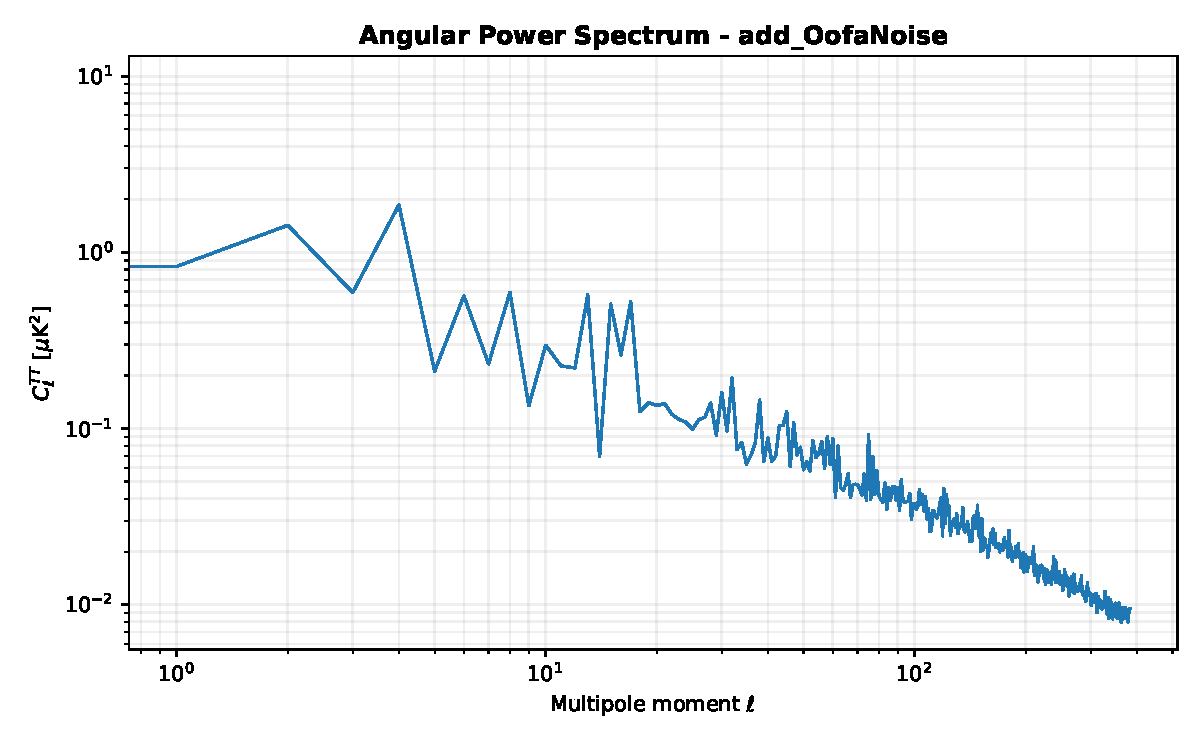
\includegraphics[width=0.65\textwidth]{psd_sh_oofa.pdf}
    \caption{Angular power spectrum using \texttt{add\_OofaNoise}.}
    \label{fig:psd_sh_oofa}
\end{figure}

The power spectra obtained for \texttt{add\_lbsNoise} (Figure 6.3) and \texttt{add\_OofaNoise} (Figure 6.4) exhibit very similar behaviors. Two main features emerge:
\begin{itemize}
    \item Low-$\ell$ Power Excess: both spectra show a marked descending slope at low multipoles. This is the signature of $1/f$ noise: long-term temporal correlations translate into large-scale spatial correlations (low multipoles) on the sky.
    \item Absence of a White Noise Plateau: in an ideal or filtered scenario, the spectrum would be expected to flatten into a plateau at high $\ell$, where white noise dominates. However, in these results, the $1/f$ noise is so predominant that it masks the white noise contribution up to the map resolution limit ($\ell \approx 350$).
\end{itemize}

The persistence of this slope is also due to the use of a simple binned map-maker. Had a destriping algorithm been applied, the low-frequency correlated components would have been suppressed, allowing the white noise plateau to emerge clearly in the spectrum. 

The comparison between the power spectra obtained for \texttt{add\_lbsNoise} and \texttt{add\_OofaNoise} reveals a strong statistical consistency between the two generation methods. Both spectra exhibit the same characteristic descending slope at low multipoles and maintain an almost identical power distribution across the entire range of $\ell$. 

